%----------------------------------------------------------------------------------------
%	PAQUETES Y OTRAS CONFIGURACIONES
%----------------------------------------------------------------------------------------

%----------------------------------------------------------------------------------------
%	PAQUETES Y OTRAS CONFIGURACIONES
%----------------------------------------------------------------------------------------

\documentclass[paper=letter, fontsize=11pt]{scrartcl} % Tamaño de papel y letra para el documento

\usepackage[utf8]{inputenc} % Los caracteres acentuados se pueden escribir normalmente en el código
\usepackage[T1]{fontenc} % Configuración de fuente de salida
\usepackage{fourier} % Se usa una fuente diferente al default
\usepackage[spanish,es-noquoting]{babel} % Se configura como documento en español
\usepackage{amsmath,amsfonts,amsthm} % Paquetes para escribir formulas matemáticas
\usepackage{graphicx} % Paquetes para incluir imágenes

\usepackage{circuitikz}
\usepackage{tikz}
\usetikzlibrary{arrows}

\usepackage{sectsty} % Paquete para configuración de secciones
\allsectionsfont{\centering \normalfont \scshape} % Los títulos de las secciones son centrados, con la misma fuente y pequeñas mayúsculas

\usepackage{todonotes}
\usepackage{microtype}

\usepackage{fancyhdr} % Paquete para personalizar pies y cabeceras de página
\pagestyle{fancyplain} % Todas las páginas con las mismas cabeceras y pies de página
\fancyhead{} % Sin cabecera
\fancyfoot[L]{} % Vacío en la izquierda del pie de página
\fancyfoot[C]{} % Vacío en el centro del pie de página
\fancyfoot[R]{\thepage} % Número de página en el pie de pagina
\renewcommand{\headrulewidth}{0pt} % Sin lineas en la cabecera
\renewcommand{\footrulewidth}{0pt} % Sin lineas en el pie de página
\setlength{\headheight}{13.6pt} % Altura de cabecera

\numberwithin{equation}{section} % Numera ecuaciones en cada sección
\numberwithin{figure}{section} % Numera figuras en cada sección
\numberwithin{table}{section} % Numera tablas en cada sección

\setlength\parindent{0pt} % Quita la indentación de los párrafos

\newcommand{\horrule}[1]{\rule{\linewidth}{#1}} % Comando personalizado para hacer linea horizontal


%----------------------------------------------------------------------------------------
%	TITULO
%----------------------------------------------------------------------------------------

\title{	
	\normalfont \normalsize
	\begin{figure}[h]
		\begin{center}
			
\includegraphics[width=0.3\textwidth]{../images/UNITEC.png}
		\end{center}
	\end{figure}
	\textsc{Instrumentación y Control} \\ [25pt]
	\horrule{0.5pt} \\[0.4cm] % Linea horizontal delgada
	\huge Práctica 1 - Sistemas eléctricos \\ % Titulo de la práctica
	\horrule{2pt} \\[0.5cm] % Linea horizontal mas gruesa
}

\author{Roberto Cadena Vega} % Nombre del profesor

\date{\normalsize 29 de mayo de 2014} % Fecha de la práctica

%----------------------------------------------------------------------------------------
%	EMPIEZA EL DOCUMENTO
%----------------------------------------------------------------------------------------

\begin{document}

\maketitle % Imprime el título

%----------------------------------------------------------------------------------------
%	OBJETIVOS
%----------------------------------------------------------------------------------------

\section{Objetivos}

	Familiarizarse con el equipo del laboratorio de electrónica y comprender el funcionamiento de circuitos eléctricos básicos.

%----------------------------------------------------------------------------------------
%	CONOCIMIENTOS PREVIOS
%----------------------------------------------------------------------------------------

\section{Conocimientos Previos}

%----------------------------------------------------------------------------------------

	\subsection{Ley de Ohm}

		La ley de Ohm es la base de cualquier modelo para un sistema eléctrico, por lo tanto nos tomamos un momento para describirla.

		\begin{equation}
			V = I \cdot R
		\end{equation}

		Donde:

		\begin{description}
			\item[$V$] Voltaje - Piensa en tus aparatos electrodomésticos; estos están diseñados para funcionar con un voltaje de $120 V$, sin embargo en el laboratorio por lo general trabajaremos con $5 V$.
			\item[$I$] Corriente - Mientras que todos tus aparatos electrodomésticos trabajan con el mismo voltaje, la corriente que utiliza cada uno será diferente (esto es lo que determina qué tanta energía gasta este aparato). Por ejemplo tu computadora puede gastar desde $2 A$ hasta $5 A$ mientras que un foco ahorrador puede utilizar $150 mA = 0.15 A$.
			\item[$R$] Resistencia - Este parámetro es lo que une al voltaje con la corriente. En el ejemplo anterior, podemos imaginar que la computadora tiene una resistencia mucho mayor al foco.
		\end{description}

		Lo que nos dice esta ley es que si tenemos un voltaje aplicado a una resistencia $V_1$, pasará a través de ella una corriente $I_1$ y tendrá el siguiente valor:

		\begin{equation}
			I_1 = \frac{V_1}{R_1}
		\end{equation}

		Recordemos también que si un circuito está en serie, todos los elementos tienen la misma corriente, es decir:

		\begin{equation}
			I_1 = I_2 = I_3 = ... = I_T
		\end{equation}

		Y que el voltaje total en un circuito en serie será la suma de todos los voltajes:

		\begin{equation}
			V_1 + V_2 + V_3 + ... = V_T
		\end{equation}

		De manera contraria, cuando tenemos un circuito en paralelo, las corrientes a través de cada uno de los elementos en paralelo se suma para obtener un total, y el voltaje en cada uno de estos elementos es el mismo

		\begin{equation}
			I_1 + I_2 + I_3 + ... = I_T
		\end{equation}

		\begin{equation}
			V_1 = V_2 = V_3 = ... = V_T
		\end{equation}

		La resistencia es diferente, cuando tenemos un circuito en serie, podemos sumar los valores de todas las resistencias para calcular la resistencia total:

		\begin{equation}
			R_1 + R_2 + R_3 + ... = R_T
		\end{equation}

		Mientras que en paralelo las resistencias no se suman tan simplemente:

		\begin{equation}
			\frac{1}{\frac{1}{R_1} + \frac{1}{R_2} + \frac{1}{R_3} + ...} = R_T
		\end{equation}

		A lo largo de la práctica se te pedirá que midas y calcules diferentes valores relacionados con la Ley de Ohm. Asegúrate de analizar primero si el circuito está en serie o en paralelo.

%----------------------------------------------------------------------------------------
%	EQUIPO
%----------------------------------------------------------------------------------------

\section{Equipo}

	El siguiente equipo será proporcionado por el laboratorio, siempre y cuando lleguen en los primeros 15 minutos de la práctica, y hagan el vale conteniendo el siguiente equipo (exceptuando las pinzas).

	\begin{itemize}
		\item Fuente de Alimentación
		\item Multímetro
		\item Cables de alimentación
		\item Pinzas
	\end{itemize}

%----------------------------------------------------------------------------------------
%	MATERIALES
%----------------------------------------------------------------------------------------

\section{Materiales}

	\begin{itemize}
		\item Protoboard
		\item LED (no importa el color, aunque los difusos son más fáciles de ver en las condiciones de iluminación del laboratorio)
		\item Resistencias
		\begin{itemize}
			\item $220 \Omega$
			\item $330 \Omega$
			\item $1 k\Omega$
		\end{itemize}
		\item Cables
	\end{itemize}

%----------------------------------------------------------------------------------------
%	DESARROLLO
%----------------------------------------------------------------------------------------

\section{Desarrollo}

    Lo primero que tenemos que hacer es realizar el circuito eléctrico en el protoboard. El circuito lo podemos ver en la figura \ref{dia:elecir}. \\

    \begin{figure}[h]
    	\begin{center}
    		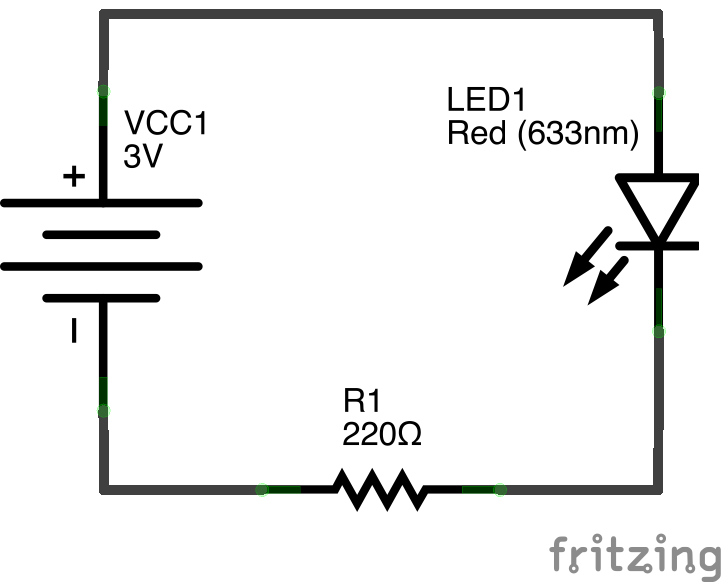
\includegraphics[width=0.3\textwidth]{images/LED-bateria-diagrama.png}
    		\caption{Diagrama eléctrico del circuito a ensamblar.}
    		\label{dia:elecir}
    	\end{center}
    \end{figure}

    Este diagrama eléctrico lo único que nos dice es que tenemos que conectar la parte positiva de nuestra batería al ánodo de nuestro LED, y el cátodo del LED, a una terminal de la resistencia. Después conectamos la otra terminal de la resistencia a la parte negativa de la batería y habremos terminado con nuestro circuito eléctrico. \\

    Pero esto aún no nos da la suficiente información para hacerlo en nuestro protoboard. Esto lo podemos ver en la figura \ref{dia:cir}. \\

    \begin{figure}[h]
    	\begin{center}
    		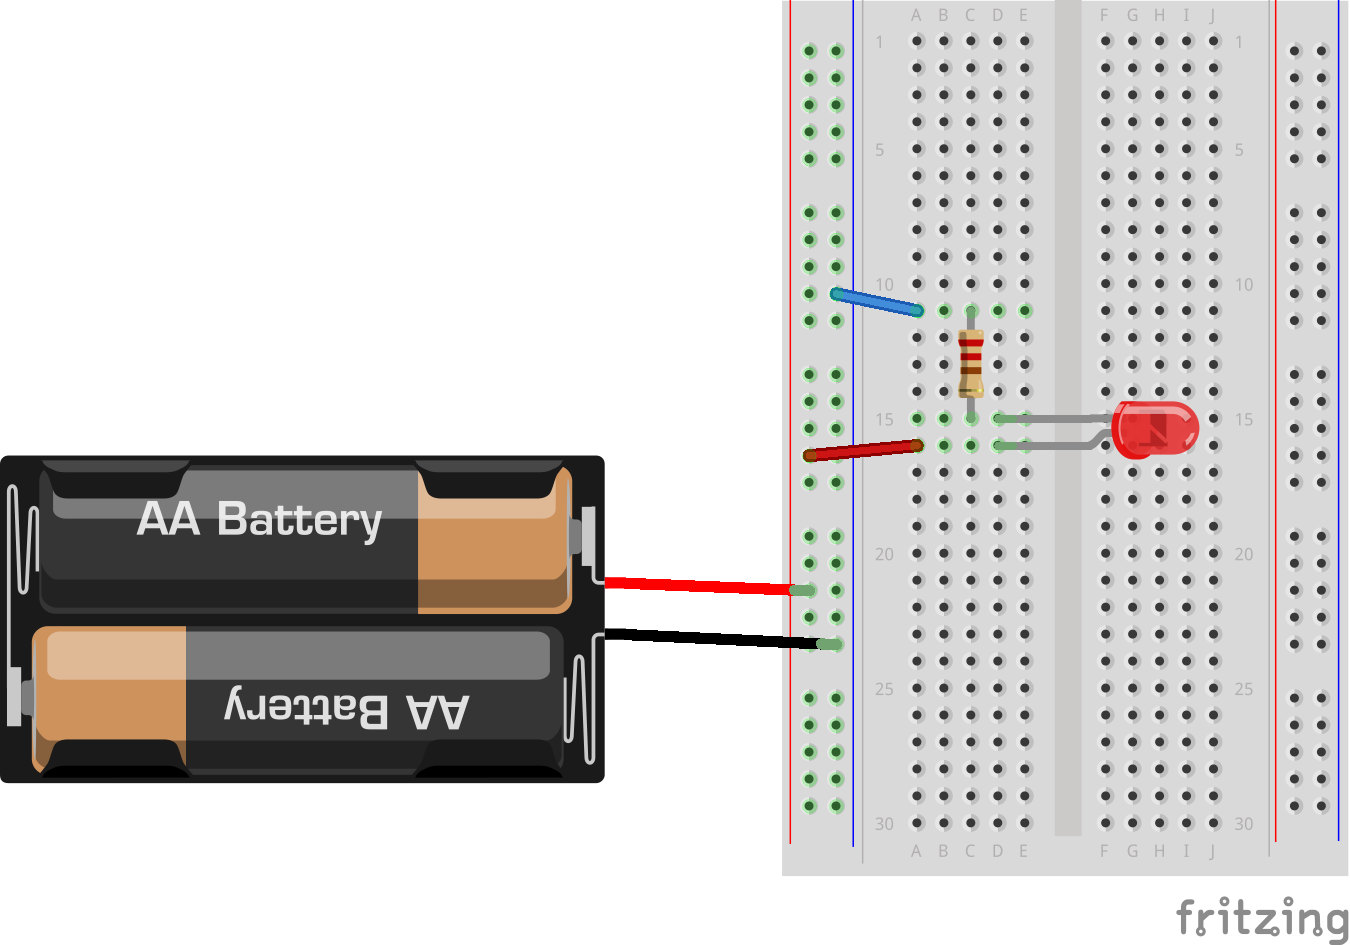
\includegraphics[width=0.5\textwidth]{images/LED-bateria.png}
    		\caption{Diagrama del circuito a ensamblar.}
    		\label{dia:cir}
    	\end{center}
    \end{figure}

    El protoboard tiene conexiones internas, que aprovechamos para hacer nuestro circuito. Primero que nada nuestro protoboard está dividido en varias partes. La parte central tiene conexiones horizontales, y las secciones laterales tienen conexiones verticales. Una práctica común es conectar el voltaje positivo de alimentación en la columna marcada de rojo en las secciones laterales y el voltaje negativo (o de referencia) en la columna marcada con azul, así siempre tenemos a la mano la alimentación en un circuito complejo (Ver la figura \ref{dia:proto}). \\

    \begin{figure}[h]
    	\begin{center}
    		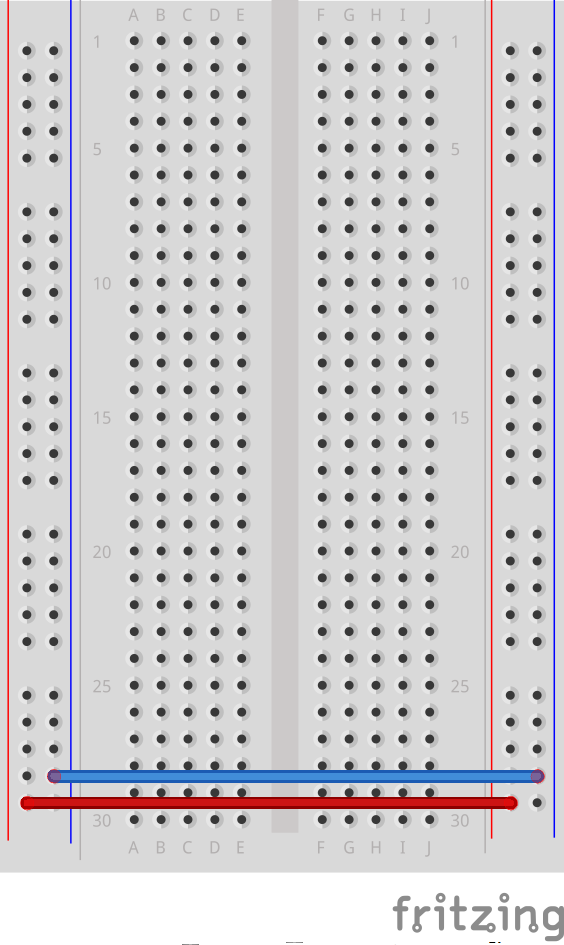
\includegraphics[width=0.25\textwidth]{images/protoboard.png}
    		\caption{Protoboard.}
    		\label{dia:proto}
    	\end{center}
    \end{figure}

    Una vez que tenemos nuestro circuito eléctrico ensamblado, podemos conectarlo a nuestra fuente de alimentación. En caso de que tengas un par de baterías AA con una manera de conectarlas, puedes hacerlo de la manera en que viene indicado en la figura \ref{dia:cir}, pero si no la has conseguido aún, no hay problema. Podemos usar la fuente de alimentación del laboratorio. \\

    Para usar la fuente de alimentación del laboratorio tenemos que asegurarnos de que esté configurada con el voltaje que queremos y que la estés conectando de la manera correcta. Por lo que te sugiero que pongas atención en la explicación que se hará en el momento de la práctica. \\

    \begin{figure}[h]
    	\begin{center}
    		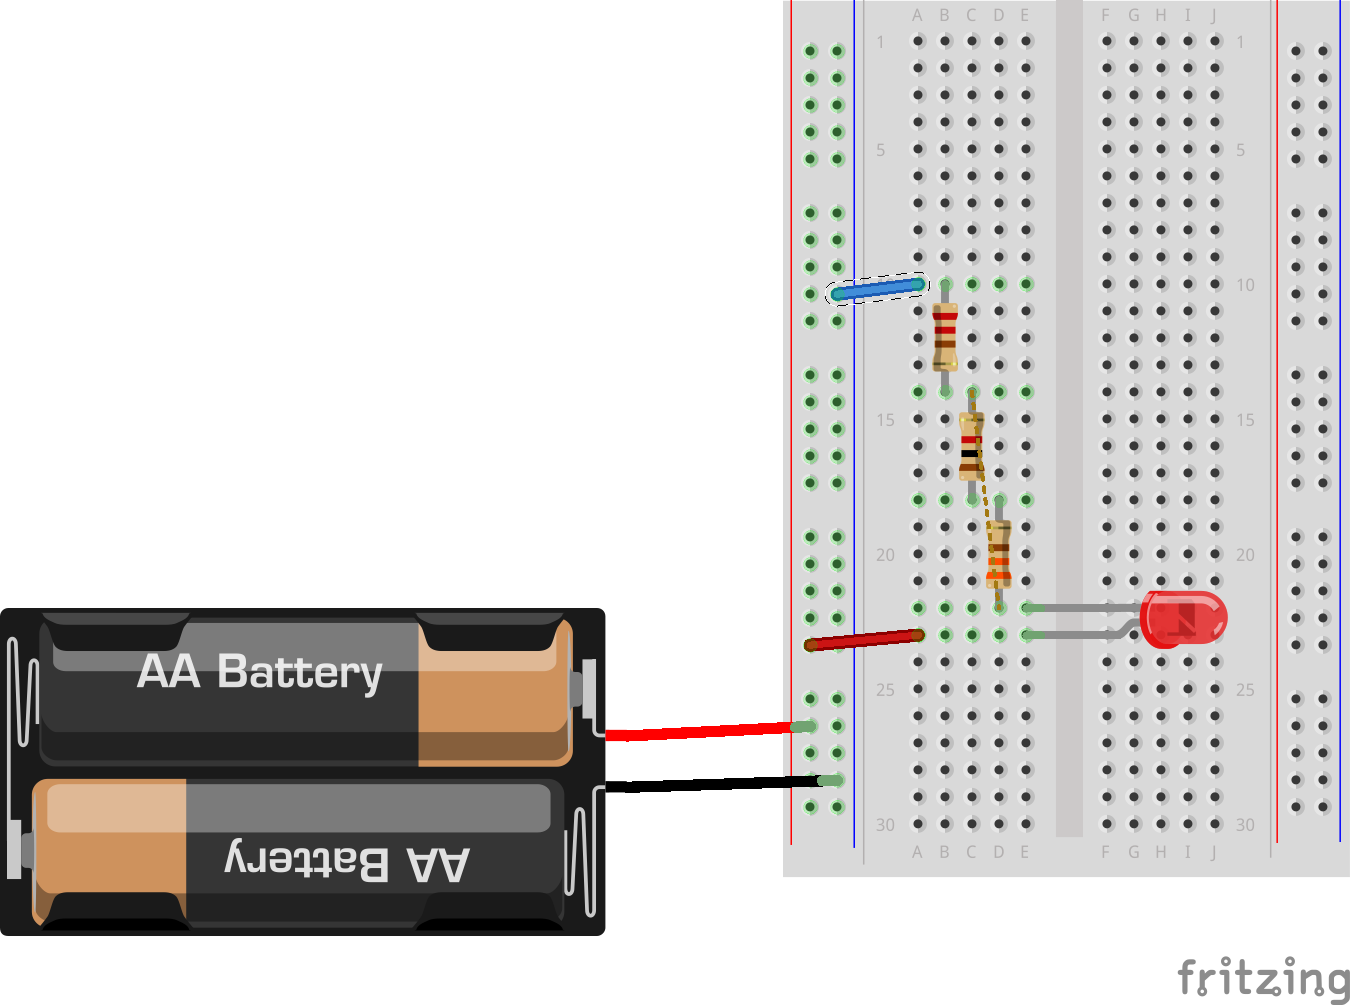
\includegraphics[width=0.5\textwidth]{images/LED-bateria-resistencias.png}
    		\caption{Diagrama del circuito eléctrico con resistencias en serie.}
    		\label{dia:serie}
    	\end{center}
    \end{figure}

    Conectado nuestro sistema a una fuente de alimentación, procederemos a medir el voltaje en la resistencia con la ayuda del multímetro. Para poder medir voltaje tenemos que configurar nuestro multímetro como Vóltmetro (esto también se explicará en la práctica). Realizamos la conexión de nuestro multímetro con las terminales de la resistencia, y en el display del multímetro estará marcado el voltaje que se aplica a la resistencia. \\

    En la figura \ref{dia:cir} se muestra una resistencia de $220 \Omega$, en la que medirás el voltaje, y calcularás la corriente; registrando cada uno de estos valores en la hoja de anotaciones que se encuentra al final de esta práctica. \\

    \begin{figure}[h]
    	\begin{center}
    		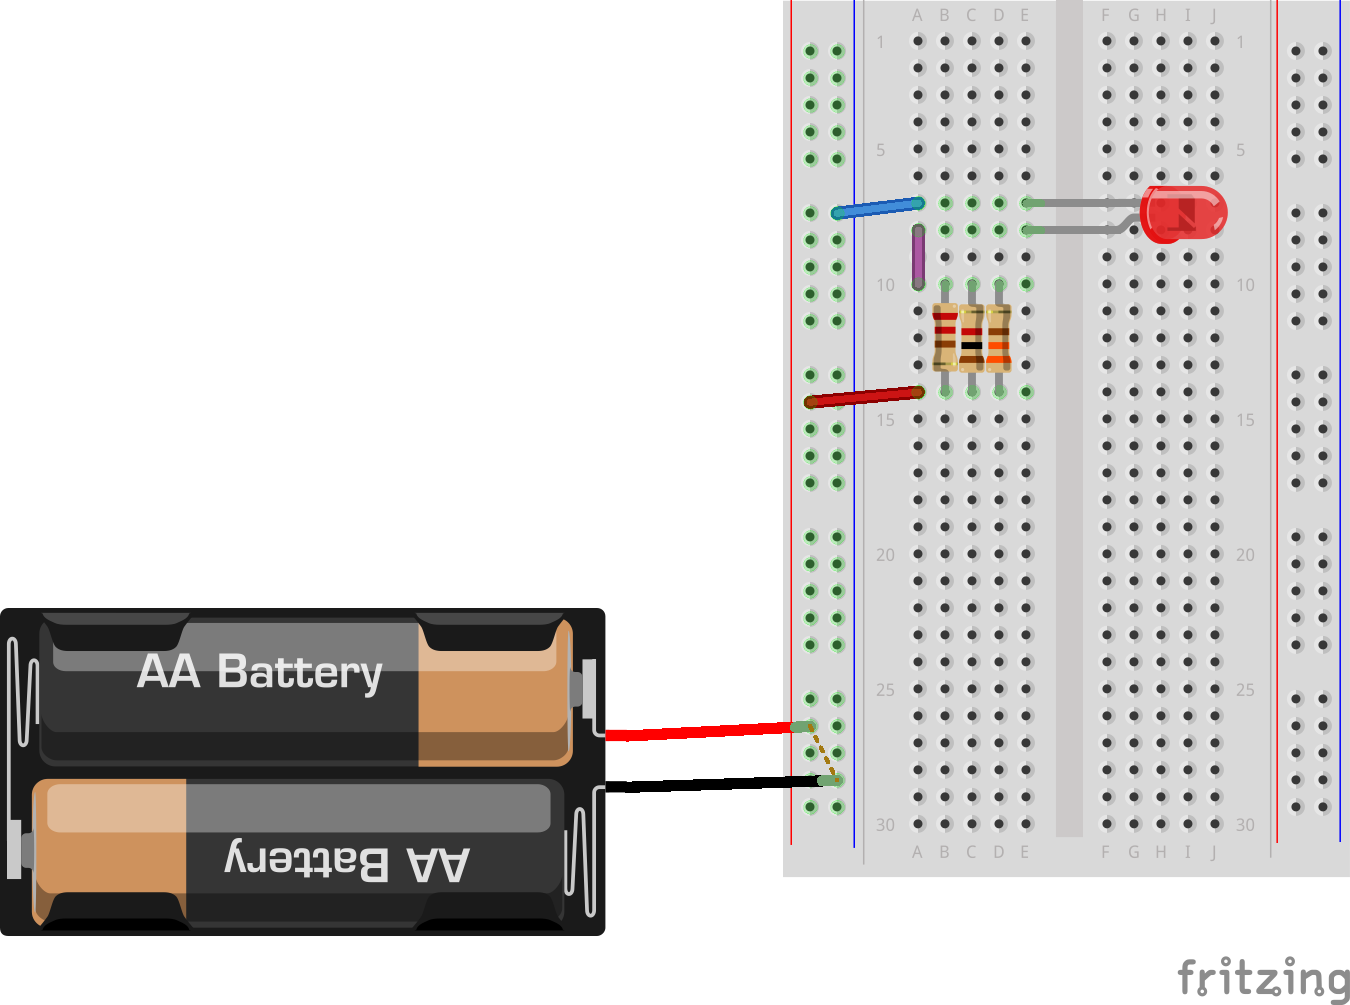
\includegraphics[width=0.5\textwidth]{images/LED-bateria-resistencias-paralelo.png}
    		\caption{Diagrama del circuito eléctrico con resistencias en paralelo.}
    		\label{dia:paralelo}
    	\end{center}
    \end{figure}

    En la segunda tabla deberás medir el voltaje aplicado en el LED, con cada una de las resistencias que has hecho el circuito. También deberás calcular la resistencia, tomando en cuenta que la corriente es la misma en la resistencia y en el LED cuando están conectadas en serie. \\

    Al terminar esta parte, tendrás que conectar en serie las tres resistencias en serie como se muestra en la figura \ref{dia:serie}. Después las conectarás en paralelo como en la figura \ref{dia:paralelo}. \\

    En la tercera tabla deberás calcular la resistencia total que se crea cuando conectas las tres resistencias en serie, y en paralelo. Medirás el voltaje y calcularás la corriente que pasa a través de tu circuito.

    Diviértete, y no dudes en preguntar al profesor cualquier duda que surja en el momento de la práctica. \\

%----------------------------------------------------------------------------------------
%	CONCLUSIONES
%----------------------------------------------------------------------------------------

\section{Conclusiones}
	El alumno deberá describir sus conclusiones al final de su reporte de práctica.

\begin{center}
	\huge \textthing
\end{center}

%----------------------------------------------------------------------------------------
%	CUESTIONARIO
%----------------------------------------------------------------------------------------

\clearpage
\section{Cuestionario - Práctica 1}
	Nombre del alumno: \\[0.2cm]
	\horrule{0.5pt} \\[0.2cm] % Linea horizontal delgada

	\begin{enumerate}
		\item Si en un circuito tenemos una corriente total de $I_T = 125 mA$ y un voltaje total de $V_T = 12 V$ ¿cuál es la resistencia total del circuito? \\ \\ \\ \\
		\item Si tenemos tres resistencias conectadas en serie, $R_1 = 180 \Omega$, $R_2 = 330 \Omega$, $R_3 = 1 k \Omega$ ¿cuál es la resistencia total? \\ \\ \\ \\
		\item ¿Y si están conectadas en paralelo? \\ \\ \\ \\
		\item ¿Qué significa ánodo? ¿Qué significa cátodo? ¿Dónde podemos ver esas partes en el LED? \\ \\ \\ \\
		\item Si tienes varios elementos conectados en paralelo ¿pasa la misma corriente por todos ellos? \\
	\end{enumerate}
    
%----------------------------------------------------------------------------------------
%	HOJA DE ANOTACIONES
%----------------------------------------------------------------------------------------

\clearpage
\section{Hoja de Anotaciones}
	Anota los pasos a seguir para utilizar correctamente la fuente de alimentación. \\ \\ \\ \\ \\ \\ \\

	Anota los pasos a seguir para utilizar correctamente el multímetro como Vóltmetro. \\ \\ \\ \\

	Realiza las mediciones de voltaje y calcula la corriente para la resistencia en el circuito:

	\begin{center}
		\begin{tabular}{|p{1.5cm}|p{1.5cm}|p{1.5cm}|}
			\hline
			$V$ & $I$ & $R$          \\
			\hline
			    &     & $220 \Omega$ \\
			\hline
			    &     & $330 \Omega$ \\
			\hline
			    &     & $1 k \Omega$ \\
			\hline
		\end{tabular}
	\end{center}

	Realiza las mediciones de voltaje y calcula la resistencia del LED en el circuito (toma en cuenta que la corriente en el LED, es la misma que en la resistencia, debido a que están conectadas en serie):

	\begin{center}
		\begin{tabular}{|p{1.5cm}|p{1.5cm}|p{1.5cm}|}
			\hline
			$V$ & $I$ & $R$ \\
			\hline
			    &     &     \\
			\hline
			    &     &     \\
			\hline
			    &     &     \\
			\hline
		\end{tabular}
	\end{center}

	Realiza las mediciones de voltaje y calcula la resistencia total de los circuitos en serie y en paralelo de resistencias. Calcula la corriente que pasa por el LED:

	\begin{center}
		\begin{tabular}{|p{1.5cm}|p{1.5cm}|p{1.5cm}|p{1.5cm}|}
			\hline
			         & $V$ & $I$ & $R$ \\
			\hline
			Serie    &     &     &     \\
			\hline
			Paralelo &     &     &     \\
			\hline
		\end{tabular}
	\end{center}

	Integrantes del equipo: \\[0.2cm]
	\horrule{0.5pt} \\[0.2cm] % Linea horizontal delgada
	\horrule{0.5pt} % Linea horizontal delgada	

	Revisó: \\[0.2cm]
	\horrule{0.5pt} \\% Linea horizontal delgada
    
%----------------------------------------------------------------------------------------
%	FIN DEL DOCUMENTO
%----------------------------------------------------------------------------------------

\end{document}